\chapter{Evaluation}

%In this chapter you should describe the previous (if possible) and final experiments performed on the implementation.

%Every single experiment should be explained individually, providing to the reader information about the meaning of the experiment, the expected %(theoretical) results, the final results, the comparison between them and others (if possible) and the conclusions. 

%Each experiment should include a description, covering (when possible) the following information:
%\begin{itemize}
%	\item Significant physical features (obstacles present on the environment, human presence, temperature, humidity, possible noise sources, computational speed of the machine, etc.)
%	\item The precise location of the experiment (latitude and longitude, room number or citation to a description of the used laboratory).
%	\item Sampling design (variable(s) measured, transformation performed to the data, samples collected, replication, comparative with a Ground Truth system, collecting data protocol).
%	\item Analysis design (how the data are processed, statistical procedures used, statistical level to determine significance).
%\end{itemize}
%The provided information should be sufficient to allow other scientists to repeat your experiment in the same conditions. Thus, the use of standard and %well-known equipment could only be represented by a simple sentence, but the non-standard equipment should be described in detail, citing the source %(vendor) and most important characteristics.

%To write it, try to use the third person when describing the experiments and results. Avoid to use first person. Past tense should be the dominant %conjugation (the work is done and was performed in the past).

%Note: Graphics represent really well data, use them! (Matlab or Octave could be useful for that).

\section{Experiment Setup}
To test the suggested approach for an RSS measurement system described in Chapter \ref{chp:apr}, the approach was implemented like described in Chapter \ref{chp:imp}. The system was then deployed and tested in the testbed described in Chapter \ref{chp:mat_testbed}. Two experiments were run. The first one was at night where no one was inside the building where the testbed is located. The second one was at daytime when there were people working inside the offices covered by the testbed and also in the other parts of the building. 

The implemented system required significant efforts in testing and debugging. Unfortunately, some bug still manifested during the execution of the collection created by message drops. This bug immediately brings the system to a stop due to discarding messages that need to be processed. Since the system directly stops when the bug occurs, it does not affect previous processes making the in the experiments measured times also valid for a fully working system. However, this made it necessary to start the system multiple times for each experiment to get as many values as possible. In the experiments, the application was restarted after half an hour to catch the stops.

To calibrate the system, 700 messages were sent with a minimum break of 20 ms. After the sink sent all its messages, it takes a 50 second break to make sure every node sent its messages. The time slot for the drops was defined as 18 ms. This is really big but when running the system inside a simulation it could be measured that the processing and sending of a message took between 5 ms and 16 ms, the extra 2 ms cover a possible error while measuring these values.  
\section{Experiment Night}
The first experiment took place at night between 02:14h and 05:54h. At this time no one was present at the whole floor. In this time, the system was restarted 7 times. Between 03:49 and 04:51 the application actually ran the whole 30 minutes and was not stopped by the mentioned bug but by the next restart. In all the other cases the application stopped during a collection. In Table \ref{tab:NightTable}, the times for each start of the application is shown as well as the overall average times for each phase. 

\begin{table}[htbp]
 \caption{Measured values for each run of the system. Time = Actual timespan in which the system took measurements; CT = Calibration Times [ms]; HOP = Number of hops inside the schedule; ST = Spread time [ms]; ACT = Average collection time [ms]; CSTD = Standard deviation of collection time [ms]; ART = Average round time [ms]; RSTD = Standard deviation of round time [ms].}
 \centering
 \begin{tabular}{c||c|c|c|c|c|c|c|c}
  Time & CT & HOP & ST & ACT & CSTD & ART & RSTD & Rounds\\ \toprule
  02:14 - 02:38 & 65611 & 44 & 784 & 3592 & 267 & 540 & 55 & 338\\
  02:45 - 02:51 & 64545 & 42 & 842 & 3637 & 280 & 519 & 38 & 73\\
  03:17 - 03:19 & 64630 & 42 & 767 & 4211 & 444 & 502 & 32 & 13\\
  03:49 - 04:19 & 64539 & 41 & 740 & 3609 & 300 & 501 & 62 & 420\\
  04:21 - 04:51 & 64565 & 44 & 804 & 3581 & 245 & 544 & 51 & 419\\
  04:53 - 04:57 & 64699 & 40 & 756 & 4287 & 343 & 429 & 48 & 35\\
  05:24 - 05:26 & 64587 & 44 & 787 & 4150 & 343 & 496 & 23 & 9\\ \toprule
  Average & 64739 & 42 & 782 & 3625 & 276 & 524 & 54 & \\
 \end{tabular}
 \label{tab:NightTable}
\end{table}

The average calibration time was 64739 ms. The time of all the different calibrations did not really change since the exact amount of messages and the break between messages is defined. It takes quite long since a huge amount of messages are sent by each node with a break up to 32 ms. Also, the break the sink takes after it sent its messages was not calculated optimally, making it possible to reduce it, resulting in a shorter calibration. When the calibration phase took roughly 64 seconds and the sink took a 50 second break after finishing sending its messages, it means the sink was finished sending its messages after 14 seconds. Now with the defined break for all the nodes in Chapter \ref{chp:imp_calibration}, we can calculate the maximal time a node needs to send all its messages. The result would be that the maximal time a node needs to send all its messages is about 40 seconds. This means the break of the sink can be reduced to around 25 seconds, reducing the overall calibration time by 25 seconds.

The average schedule has 42 hops meaning that 42 messages need to be sent in one round the schedule takes. The schedule with the largest amount of hops has 44 and the smallest has 40 hops. The different schedules emerge through different measured RSS values while calibrating.

Spreading the schedule took in average 782 ms. This is fast since a schedule of 40+ hops needs two messages to be sent. This means that spreading one schedule part inside the whole network took around 390 ms.

The collection of the gathered information took averagely 3625 ms with an average standard deviation of 276 ms. Compared to the spreading of the schedule, this is really slow. However, we need to take into account that the collection requires more messages and processing than the spreading. To analyze if the time of the collection changes during the course of time and if a new calibration is needed, Figure \ref{fig:nightC} shows the times of all the collections between 03:49h and 04:19h. However, the Figure does not show any significant change over the 30 minutes of time indicating that there would be no new calibration necessary to maintain performance of the application.

\begin{figure}[htbp]
	\centering         
    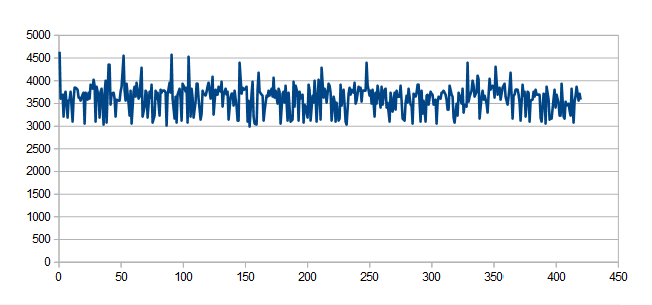
\includegraphics[scale=0.75]{content/images/Experiment/NightCollection}
    \caption{Collection times of the measurements from 03:49h to 04:19h.}
	\label{fig:nightC}
\end{figure}

Sending all the messages for one round takes in average 524 ms with an average standard deviation of 54 ms. Again we want to analyze if the round time changes during the course of time. Therefore the round times of all the rounds between 03:49h and 04:19h are shown in Figure \ref{fig:nightR}. Again we do not see a significant change in the time one round takes. This means that message drops do not increase over the 30 minutes.

\begin{figure}[tbp]
	\centering
	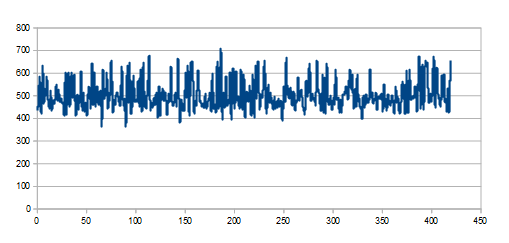
\includegraphics[scale=0.75]{content/images/Experiment/NightRounds}
 	\caption{Sampling times of the measurements from 03:49h to 04:19h.}
	\label{fig:nightR}
\end{figure}

\section{Experiment Day}
The second experiment took place from 09:32h to 14:17h. In this timespan the application was started and restarted 9 times. The first person arrived at 09:00h, the second at 10:00h, the third at 11:20h, the forth at 13:00h and the last one at 13:30. Moreover one person arrived and left sometime between 10:30h and 12:30h. Moreover one left at 12:00h. All these people where working in their offices.
The results of the experiment are shown in Table \ref{tab:DayTable}
\begin{table}[htbp]
 \caption{Measured values for each run of the system. Time = Actual timespan in which the system took measurements; CT = Calibration Times [ms]; HOP = Number of hops inside the schedule; ST = Spread time [ms]; ACT = Average collection time [ms]; CSTD = Standard deviation of collection time [ms]; ART = Average round time [ms]; RSTD = Standard deviation of round time [ms].}
 \centering
 \begin{tabular}{c|c||c|c|c|c|c|c|c|c}
  Time & Persons & CT & HOP & ST & ACT & CSTD & ART & RSTD & Rounds\\ \toprule
  09:32 - 09:38 & 1 & 64647 & 43 & 823 & 4401 & 296 & 492 & 41 & 63\\ 
  10:04 - 10:14 & 2 & 64558 & 44 & 796 & 4035 & 322 & 563 & 59 & 121\\
  10:36 - 10:53 & 2 & 64644 & 41 & 850 & 3740 & 282 & 482 & 40 & 231\\
  11:07 - 11:09 & 2 & 64577 & 41 & 849 & 3746 & 423 & 533 & 60 & 14\\ 
  11:39 - 12:09 & 3-2 & 64607 & 39 & 797 & 3498 & 358 & 495 & 42 & 433\\
  12:11 - 12:28 & 2 & 64654 & 41 & 764 & 3556 & 294 & 495 & 45 & 240\\
  12:43 - 13:13 & 2-3 & 64583 & 44 & 824 & 4160 & 511 & 539 & 65 & 368\\
  13:15 - 13:29 & 3 & 64544 & 44 & 797 & 3697 & 398 & 542 & 58 & 183\\
  13:47 - 13:53 & 4 & 64580 & 41 & 778 & 3494 & 371 & 528 & 46 & 73\\ \toprule
  Average & & 64599 & 42 & 809 & 3773 & 372 & 514 & 50 & \\
 \end{tabular}
 \label{tab:DayTable}
\end{table}

Since the mean values of both experiments fall in each others standard deviation, it seems that typical activities in an indoor environment do not impact the functioning of the approach. Again we look at the individual times of the collection from 11:39h to 12:09h in Figure \ref{fig:dayC} to see if they change over time. In general, the time for a collection does not increase over time, however at around collection 400 we can see a huge deviation. Here the collection once takes 5186 ms and once 7293 ms. After that the collection time normalizes again. This deviation could indicate that at that point in time a, for the links inside the testbed, huge change in the environment caused a lot of message drops creating this long collection. Most likely this change was created by the person leaving at around 12:00h. It left the floor by using the elevator which has a huge impact on the links in the testbed.


\begin{figure}[htbp]
	\centering         
    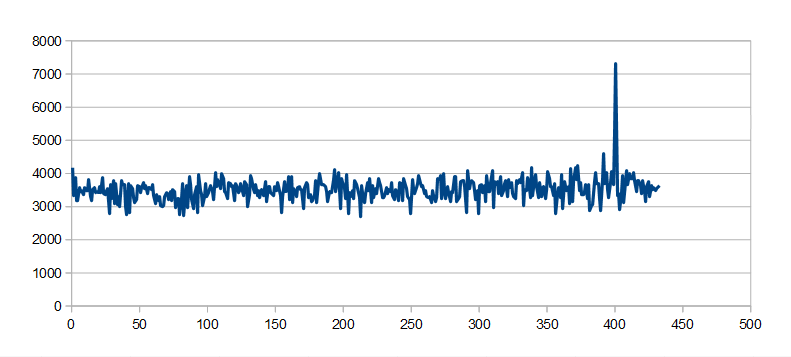
\includegraphics[scale=0.75]{content/images/Experiment/DayCollection}
    \caption{Collection times of the measurements from 11:39h to 12:09h.}
	\label{fig:dayC}
\end{figure}

In Figure \ref{fig:DayR}, we take a look at the individual times of the rounds between 11:39h and 12:09h. Here we can see slight fluctuations of the time. However we cannot say if these are created by decalibration or higher activity by the persons inside the offices. For example, increase of time starting at round 300 can also be created by the person leaving since it started walking around.

\begin{figure}[tbp]
	\centering
    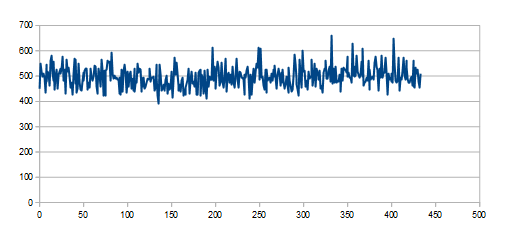
\includegraphics[scale=0.75]{content/images/Experiment/DayRounds}
   	\caption{Sampling times of the measurements from 11:39h to 12:09h.}
    \label{fig:DayR}
\end{figure}
    

\section{Usability for RTI Localisation}
The experiments show that the system is usable in an office environment and delivers one full RSS measurement averagely every 4 seconds. The measurements are fast enough to detect a moving person. The long collection phase creates jumps of 3.5 seconds between each measurement. In that time a person can move a lot and could make the tracking of the person difficult. However it could be possible to have multiple measurement rounds before collecting the data. This could improve the tracking.

\section{Comparison to a Time Slot Based Approach}
The approach suggested by this thesis tries to improve a fully time slot based approach like Multi-Spin by defining predecessors and successors for each node to eliminate the error included in a timeslot. 
These two approaches can be compared by calculating the time a round would need. Therefore we assume that a time slot based system would choose the same time slot size as the predecessor successor approach to catch message loss.

In the experiments, a time slot of 18 ms was used to catch message loss. There are 32 nodes inside the network, meaning a time slot based approach would need 576 ms for one round. The average time a round needed in the experiments was around 520 ms which is actually faster although there are in average 10 messages more that need to be sent with the successor predecessor approach. This advantage could be improved even more by optimizing the schedule, shrinking the amount of messages that need to be sent in one round.  

An advantage of the time slot based approach would be that rounds have a very stable time. The average round time in the experiments is indeed faster than the time of a time slot based system, however the round time fluctuates, meaning that the times range from around 370 ms to around 640 ms. Depending on the purpose of the application, a stable time could be preferred over the faster average time. Moreover, in a time slot based system, it is not possible that one node does not send a message while in the successor predecessor approach it can happen that a node does not send a message when it never received a message until it is its turn. However this should happen rarely.